\chapter{Lab and place}
\section{The MIVIA Laboratory}

\begin{wrapfigure}[2]{l}{2cm}
	\vspace{-7mm}
	
\includegraphics[width=2cm]{images_not_compressed/MIVIALogo.jpg}
	\end{wrapfigure}
 for Macchine Intelligenti per il riconoscimento di Video, Immagini e Media which means intelligent machines for video, images and media recognition. The laboratory is located in Fisciano, Campania, Italy, near Salerno and Napoli as we can see below.
 \begin{figure}[h]
 \begin{center}
	 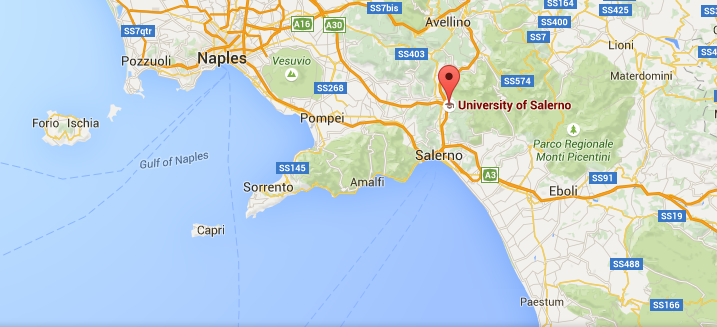
\includegraphics[width=12cm]{images_not_compressed/geoUniversity.png}
		\caption{Location of the University}
	 \end{center}
 \end{figure}
 \par As its name suggests it, except theaching computer sciences, doctors of the lab work on pattern recognition, classification, media analysis and many parallele subjects like autonomus drones and robot vision.
 \par The laboratory is directed by Mario Vento. He is assisted by Alessia Saggese. Pasquale Foggia, Gennaro Percannella and Pierluigi Ritrovato (who is also my tutor) are teachers and researchers for the lab. There are also several students and graduated that work on thesis for the laboratory. I was more in contact with Antonio Greco and Raffaele Iuliano. All students and graduated was working on differents projects and start-ups. And the laboratory itself works for and with international companies.
 \par You can find all of this information on their website at this address : \url{http://mivia.unisa.it/}
 \par Because of the opportunity of double diploma, the proximity with France, the possibility to learn a new language even if I know that everybody speaks english between us. I was really optimistic about the place and the laboratory.
	 
 \section{Place and life in Italy}
 
 \par The first month of internship, I lived in Carpineto, 25 minutes to the university by foot. It was envoying the view on the montains in the morning and the evening but when I wanted to move the week-end, buses didn't pass near my flat so that I had easily hours of walk to get back home. I moved on to Salerno, in the centro historico. Than it was easier to move the week-ends. 
 \par The main tourstic place around is the Amalfitan coast which is really beautiful. There is also Napoli and Pompei which are really near. There is also a lot of beaches and montains. A really nice place where you can have snow in the winter and 33 degrees during weeks in the summer. 
  \begin{figure}[h]
 \begin{center}
	 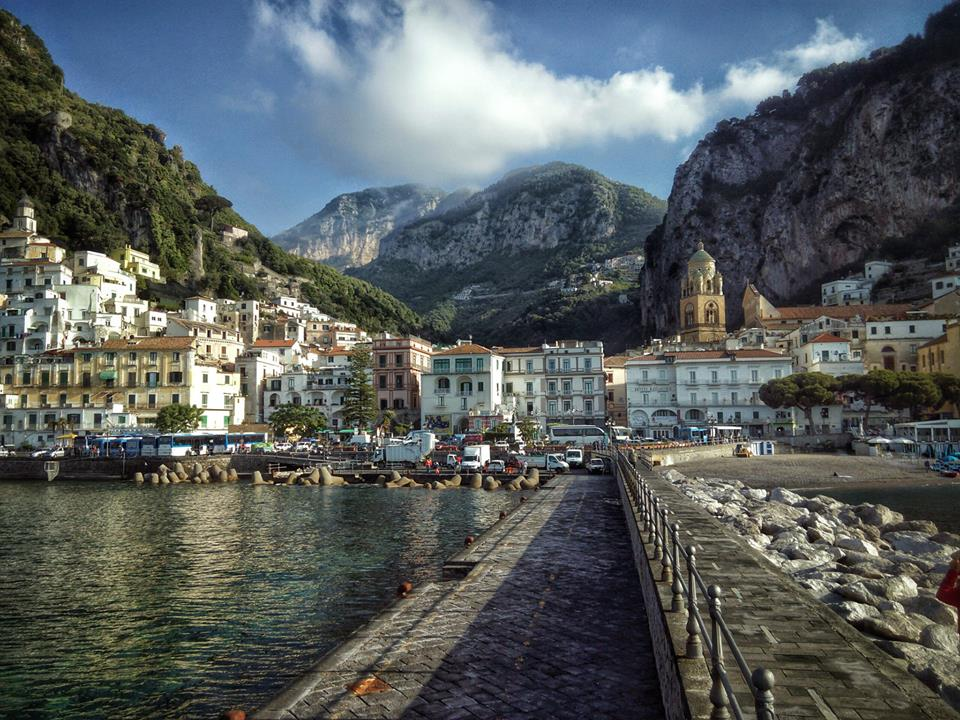
\includegraphics[width=12cm]{images_not_compressed/amalfi.jpg}
		\caption{Picture of Amalfi early in the morning from the harbour}
		\label{amalfi}
	 \end{center}
 \end{figure}

 \par In the picture~\ref{amalfi} the beach is not set for summer so there is nowone, but in july, it becomes overcrowded because of tourism. Also, I found that this part of Italy is really human. It feels like you can trust people really quickly because they are really sympathics. In that way, there is few offical contract. That is suprising when you come from France and it requires a thousand of documents to get a flat. Here, the ID card is enough. People are always happy but a bit slow when the walk that is getting on my nerves when I am in a hury.
 I took advantage of the intership to make a lot of trekking in the amalfitan coast and around Fisciano. Visite ruins, Napoli and see a lot of churches because christianism is really present in Italy.